
%%%%%%%%%%%%%%%%%%%%%        PERSONNAGE AU BORD D'UNE MARE
%  DÉFINITIONS

\tikzset{
  feuillage/.style = {decoration={random steps, segment length=0.4mm}, decorate},
  tronc/.style   = {decoration={random steps, segment length=2mm, amplitude=0.2mm}, decorate}}

\tikzset{  arbre/.pic={ \foreach \w/\f in {0.3/30,0.2/50,0.1/70} { \fill [brown!\f!black, tronc] (-\w/2,0) rectangle +(\w,3); } \foreach \n/\f in {1.4/40,1.2/50,1/60,0.8/70,0.6/80,0.4/90} { \fill [green!\f!black, feuillage](0,3) ellipse (\n/1.5 and \n); }}}

\tikzset{  personnage/.pic={ { \fill [black] (0,0)ellipse(0.25 and 0.55); } 
  { \fill [black](0,0.75)circle(0.2); }
    % jambe et pieds
  {\fill [rounded corners=2pt] (0.1,-0.3)rectangle(-0.1,-1.5);}
  {\fill [rounded corners=2pt] (0.3,-1.4)rectangle(-0.1,-1.5);}
    % bras
  {\fill [rounded corners=2pt, rotate=-15] (-0.1,0.42)rectangle(0.5,0.29);}
  {\fill [rounded corners=2pt] (0.44,0.17)rectangle(1,0.29);}}}

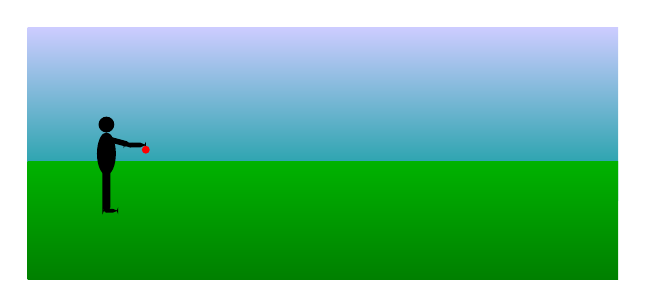
\begin{tikzpicture}%[scale=0.5]
    %  Ciel
  \shade[bottom color=cyan!60!black, top color=blue!20!white] (0,0) rectangle (7.5,2.2);
    %  Sol
  \shade[bottom color=green!50!black, top color=green!70!black] (0,0.5) rectangle (7.5,-1);
    %  Mare
 % \shade[bottom color=blue!50!white, top color=cyan!60!black] (3.7,-0.15) ellipse (2.5 and 0.3);
    %  Arbre
 % \pic at (2,2)    {arbre};

    %  Personnage
  \begin{scope}[xshift=1 cm,yshift=0.6 cm]
    % corps et tête
 \fill [black] (0,0)ellipse(0.12 and 0.27);
 \fill [black](0,0.37)circle(0.1);
    % jambe et pieds
 \fill [rounded corners=2pt] (0.05,-0.15)rectangle(-0.05,-0.75);
 \fill [rounded corners=2pt] (0.15,-0.7)rectangle(-0.05,-0.75);
    % bras
 \fill [rounded corners=2pt, rotate=-15] (-0.1,0.22)rectangle(0.28,0.15);
 \fill [rounded corners=2pt] (0.22,0.08)rectangle(0.5,0.14);
   % Balle
 \fill[red] (0.5,0.05) circle(0.05);
  \end{scope}

\end{tikzpicture}

%%%%%%%%%%%%%%%%%%%%%%%%%%%%%%%%%%%%%%%%%%%%%%%%%%%%%%%%%%%%%%%%%%%%%%%%%%%%%%%%
